\documentclass[a4paper,11pt]{article}
\usepackage{fontspec}
\setmainfont{Times New Roman}
\setsansfont{Arial}
\usepackage[margin=23mm,headheight=14pt]{geometry}
\usepackage{amsmath,amssymb,bm,booktabs,array,tabularx,graphicx,float,placeins,multirow}
\usepackage{tikz}
\usetikzlibrary{arrows.meta,positioning}
\usepackage{enumitem,caption,fancyhdr}
\usepackage{xr-hyper}
\usepackage[unicode,hidelinks]{hyperref}
\setlength{\parskip}{0.25em}
\setlength{\emergencystretch}{3em}
\raggedbottom
\renewcommand{\topfraction}{0.92}
\renewcommand{\bottomfraction}{0.9}
\renewcommand{\textfraction}{0.06}
\renewcommand{\floatpagefraction}{0.85}
\setcounter{topnumber}{4}
\setcounter{bottomnumber}{3}
\makeatletter
\setlength{\@fptop}{0pt}
\setlength{\@fpsep}{16pt}
\setlength{\@fpbot}{0pt plus 1fil}
\makeatother
\renewcommand{\arraystretch}{1.18}
\captionsetup{font=small,labelfont=bf}
\setlist{nosep,leftmargin=2em}
\pagestyle{fancy}\fancyhf{}
\fancyfoot[C]{\thepage}
\newcommand{\R}{\mathbb{R}}
\newsavebox{\fulltablebox}
\newcommand{\method}{\textbf{MetaMatch-TTA}}
\newcommand{\matcher}{\textbf{MetaMatch}}
\newcommand{\sigmoid}{\operatorname{sigmoid}}
\newcommand{\clip}{\operatorname{clip}}

\hypersetup{pdftitle={Background-Aware Hyperspectral Target Detection with Mismatched Reference Spectra - Supplementary Material},pdfauthor={},pdfsubject={Supplementary material}}
\fancyhead[L]{\small MetaMatch-TTA}\fancyhead[R]{\small Supplementary material}
\externaldocument[][nocite]{research_manuscript_en}
\renewcommand{\thesection}{S\arabic{section}}
\renewcommand{\thetable}{S\arabic{table}}
\renewcommand{\thefigure}{S\arabic{figure}}
\renewcommand{\theequation}{S\arabic{equation}}
\renewcommand{\thepage}{S\arabic{page}}
\title{\bfseries Background-Aware Hyperspectral Target Detection with Mismatched Reference Spectra\\[0.6em]{\large Supplementary Material}}
\author{}
\date{}
\begin{document}
\maketitle
\vspace{-2.5em}
\section{Component Ablations of the Direct Matcher}\label{supp:ablation}
Direct-matching ablations identify component contributions before reference updates. The experiments use development split A, for which complete records are available. AVIRIS-2, SanDiego2, and ABU-A2 are used for training, while Segundo, Cri, and ABU-B4 are used for evaluation. The three configurations share the training budget, seed 0, and reference draws. The complete model is paired with models without augmentation and without whitened sequence channels. This setup isolates the behavior of the shared matching function.

\begin{table}[htbp]\centering\scriptsize\setlength{\tabcolsep}{4pt}
\caption{Ablations of \textbf{\matcher{}} on held-out development scenes. Each entry averages three reference draws with one training seed. The highest value within P1 and P4 for each scene is bold. Removing whitened channels retains the associated scalar features.}\label{tab:ablation}
\begin{tabular}{lrrrrrr}\toprule & \multicolumn{3}{c}{\textbf{\matcher} (P1)} & \multicolumn{3}{c}{\textbf{\matcher} (P4)} \\
\cmidrule(lr){2-4}\cmidrule(lr){5-7}
Scene & \textbf{Full model} & w/o aug. & \shortstack{w/o whitened\\channels} & \textbf{Full model} & w/o aug. & \shortstack{w/o whitened\\channels} \\
\midrule
Segundo & 0.9758 & \textbf{0.9900} & 0.9844 & 0.9922 & 0.9914 & \textbf{0.9939} \\
Cri & \textbf{0.9993} & 0.9241 & 0.9462 & \textbf{0.9994} & 0.9684 & 0.9720 \\
ABU-B4 & \textbf{0.9163} & 0.8881 & 0.8308 & \textbf{0.9355} & 0.9233 & 0.8932 \\
\bottomrule
\end{tabular}
\end{table}

Table~\ref{tab:ablation} directly tests pairwise discrimination before candidate updates. On Cri under P1, the complete model achieves 0.9993, exceeding the 0.9241 obtained without augmentation by 7.52 percentage points. On ABU-B4, the complete result of 0.9163 exceeds the configurations without augmentation and without whitened channels by 2.82 and 8.55 percentage points, respectively. Neither image participates in training for this split, so the improvements reflect the role of these components in judging material relationships in new images. Augmentation exposes same-material matching to different observation forms, while whitened channels condition similarity on current-background statistics. These components already contribute during the first image-wide scoring pass, providing more discriminative candidates for subsequent reference updates.

The complete configuration obtains the highest ROC-AUC in four of the six direct-matching comparisons, corresponding to P1 and P4 on Cri and ABU-B4. On Segundo, the complete, no-augmentation, and no-whitened-channel configurations achieve 0.9758, 0.9900, and 0.9844 under P1, and 0.9922, 0.9914, and 0.9939 under P4. Component gains therefore vary with the material task. Since the no-whitened-channel configuration retains analytical scalars, this ablation specifically evaluates the incremental information in the whitened sequence channels. Together with the refined-stage results on the same scenes, the direct ablations support encoding tolerance to spectral variation and background-relative relationships in the shared matcher.


\section{Implementation Settings and Randomness}\label{supp:implementation}
Table~\ref{tab:config} summarizes the unified configuration for reusing the network across scenes. Nine-channel sequences and four analytical statistics jointly supply material relationships and scene conditions to the matcher. Sequence pooling keeps the prediction-head dimensions fixed, and two reference updates bound the number of online adaptation iterations. All reference protocols use the same network, candidate ratio, and training budget, so differences in results reflect changes in input information and output stage. This unified interface reduces the need to construct separate detectors for different band counts or reference budgets, implementing the combination of background-conditioned matching and fixed-weight reference adaptation.
\begin{table}[htbp]\centering\small\setlength{\tabcolsep}{4pt}
\caption{Implementation settings of \textbf{\method{}}.}\label{tab:config}
\begin{tabularx}{\linewidth}{p{4cm}X}\toprule
Item & Setting \\ \midrule
Sequence and scalar inputs & Nine-channel spectral pair sequence and four analytical statistics \\
Network width and pooling & Width 64, with attention-weighted mean, ordinary mean, and maximum pooling \\
Material tasks & 40 clusters, retaining clusters of at least 30 pixels; 64 positive and 192 negative samples per task \\
Task supervision & Primarily clustering tasks, with development target labels used with probability 0.2 \\
Optimization & AdamW for 2,000 steps, accumulating four tasks per step, with peak learning rate $10^{-3}$ \\
Positive-class weight / weight decay & 2 / $10^{-4}$ \\
Image whitening & Covariance shrinkage coefficient 0.05 and eigenvalue floor $10^{-10}$ \\
Reference refinement & Two updates, candidate ratio 0.002, and candidate count clipped to $[5,200]$ \\
Training randomness & Training seeds 0, 1, and 2 \\
Reference randomness & Draw index $\mathrm{draw}\in\{0,1,2\}$, with reference-generation seed $1000+\mathrm{draw}$ \\
\bottomrule\end{tabularx}
\end{table}

\begin{table}[htbp]\centering\small\setlength{\tabcolsep}{4pt}
\renewcommand{\arraystretch}{1.02}
\caption{Training-seed-specific ROC-AUC of \textbf{\method{}}. Each entry averages the same three reference draws. The highest seed result for each scene within each protocol is bold. Main results average the three seeds.}\label{tab:seeds}
\begin{tabular}{lrrrrrr}\toprule & \multicolumn{3}{c}{\textbf{\method} (P1)} & \multicolumn{3}{c}{\textbf{\method} (P4)} \\
\cmidrule(lr){2-4}\cmidrule(lr){5-7}
Scene & Seed  0 & Seed  1 & Seed  2 & Seed  0 & Seed  1 & Seed  2 \\
\midrule
ABU-A3 & 0.9712 & 0.9742 & \textbf{0.9787} & 0.9710 & \textbf{0.9759} & 0.9745 \\
ABU-B3 & 0.9868 & \textbf{0.9879} & 0.9801 & \textbf{0.9887} & 0.9867 & 0.9763 \\
ABU-U4 & \textbf{0.9971} & 0.9968 & \textbf{0.9971} & \textbf{0.9975} & 0.9972 & 0.9974 \\
SanDiego & 0.9891 & \textbf{0.9934} & 0.9917 & \textbf{0.9944} & 0.9938 & 0.9937 \\
HYDICE & \textbf{0.9984} & 0.9967 & 0.9963 & \textbf{0.9990} & 0.9969 & 0.9973 \\
WHR & 0.9955 & \textbf{0.9971} & 0.9964 & 0.9943 & \textbf{0.9959} & 0.9948 \\
\bottomrule
\end{tabular}
\end{table}

Table~\ref{tab:seeds} examines whether high accuracy depends on a particular training initialization. On ABU-U4, the three seeds yield 0.9968--0.9971 under P1 and 0.9972--0.9975 under P4. The range across seeds is 0.03 percentage points in both cases. The corresponding ranges on HYDICE are 0.9963--0.9984 and 0.9969--0.9990, with high target-ranking accuracy for all three seeds. Detection capability with single-pixel and perturbed references therefore recurs across training runs. The main tables use equal-weight seed means, incorporating this repeatability alongside reference sampling and supporting stable discrimination through randomized-reference task learning.


\section{Protocol Summary and Student Controls}\label{supp:student}
Table~\ref{tab:protocols} summarizes macro-average ROC-AUC for the same matcher under all reference conditions. \method{} improves from 0.9902 with a single pixel to 0.9924 with a five-pixel mean, matching the complete-mean result at the reported precision. The model can therefore use additional observations to improve the target description. Direct matching achieves 0.9914 under P4, showing that tolerance to the synthetic changes is established before reference adaptation. Evaluating reference count and spectral variation within one fixed network supports the use of material-task learning to reduce dependence on a particular reference construction.
\begin{table}[H]\centering\footnotesize\setlength{\tabcolsep}{4pt}\renewcommand{\arraystretch}{1.14}
\caption{Scene-macro-average ROC-AUC of \matcher{} and \method{} under the reference protocols. All values are measured in this study. The highest value in each row is bold.}\label{tab:protocols}
\begin{lrbox}{\fulltablebox}\begin{tabular}{lcc}\toprule
Protocol & \textbf{\matcher{}} & \textbf{\method{}} \\ \midrule
P0 & \textbf{0.9925} & 0.9924 \\
P1 & 0.9895 & \textbf{0.9902} \\
P2 ($k=3$) & \textbf{0.9900} & 0.9899 \\
P2 ($k=5$) & 0.9922 & \textbf{0.9924} \\
P4 & \textbf{0.9914} & 0.9903 \\
P3 & \textbf{0.9891} & 0.9874 \\
\bottomrule\end{tabular}\end{lrbox}\ifdim\wd\fulltablebox>\linewidth\resizebox{\linewidth}{!}{\usebox{\fulltablebox}}\else\usebox{\fulltablebox}\fi\end{table}

The student control takes $[\widetilde x_i,\widetilde x_i\odot\widetilde d]$ as input to a perceptron with two hidden layers of width 128. It is trained against refined soft scores for 40 epochs using Adam with learning rate $10^{-3}$. Sample weights are $0.2+0.8|2s_i-1|$, and student and teacher scores are averaged equally. In Table~\ref{tab:stages}, direct matching, reference refinement, and fusion achieve 0.9895, 0.9902, and 0.9905 under P1, respectively. With five-pixel references, they achieve 0.9922, 0.9924, and 0.9919. Gradient-free updates already improve average accuracy in both limited-reference settings, whereas the student adds a gain only under P1. Direct matching yields the highest P4 value of 0.9914, showing that tolerance to the prescribed spectral variations does not depend on student fitting. Timing records include the student, diagnostic branches, and metric computation, with background preprocessing completed before timing starts. This comparison supports fixed-network material discrimination and reference adaptation as the main pipeline, with scene-specific learning evaluated as a separate extension.
\begin{table}[H]\centering\small\setlength{\tabcolsep}{4pt}
\renewcommand{\arraystretch}{1.02}
\caption{Macro-average ROC-AUC of \textbf{\matcher{}}, \textbf{\method{}}, and the student-fusion control. The highest value in each row is bold. Student fusion is not required by the main method.}\label{tab:stages}
\begin{tabular}{lrrr}\topruleProtocol & \textbf{\matcher} & \textbf{\method} & \shortstack{\textbf{\method}\\+Student fusion} \\
\midrule
P0 & \textbf{0.9925} & 0.9924 & 0.9924 \\
P1 & 0.9895 & 0.9902 & \textbf{0.9905} \\
P2($k=3$) & \textbf{0.9900} & 0.9899 & \textbf{0.9900} \\
P2($k=5$) & 0.9922 & \textbf{0.9924} & 0.9919 \\
P4 & \textbf{0.9914} & 0.9903 & 0.9896 \\
P3 & \textbf{0.9891} & 0.9874 & 0.9887 \\
\bottomrule
\end{tabular}
\end{table}
\FloatBarrier


\section{Complementary Development Splits}\label{app:development}
Two complementary development splits test whether material relationships transfer from three training scenes to three other scenes. Each split uses training seed 0, and held-out images participate only in evaluation for that split. Table~\ref{full:tab:dev} and Fig.~\ref{full:fig:dev} organize the results by output stage and reference condition. Separating fitting on available images from matching on new images directly evaluates the transferability of shared relationships.

Across 27 scene--protocol combinations, \method{} achieves ROC-AUC values of 0.8062--0.9996, with seven combinations reaching at least 0.99. Cri achieves 0.9994--0.9996 across reference conditions, indicating that its material relationships can be learned from other scenes and remain stable as references change. ABU-A2 obtains 0.8489 under P0 and 0.8062 under P2, showing that transfer across materials also depends on training-task coverage and target--background similarity. Retaining these task differences helps identify both the capabilities already acquired by the shared matcher and priorities for expanding material coverage.

\begin{table}[H]\centering\footnotesize\setlength{\tabcolsep}{4pt}\renewcommand{\arraystretch}{1.12}
\caption{ROC-AUC on two complementary development splits. Each split uses three training scenes, three held-out scenes, and training seed 0. Entries average up to three references according to the existing protocol. The highest value in each row is bold. The student and its fused output are separate controls.}\label{full:tab:dev}
\begin{lrbox}{\fulltablebox}\begin{tabular}{llcccc}\toprule
Protocol & Scene & \textbf{MetaMatch} & \textbf{MetaMatch-TTA} & \textbf{Student} & \shortstack{\textbf{MetaMatch-TTA}\\+S} \\ \midrule
P0 & Segundo & 0.9932 & 0.9938 & 0.9940 & \textbf{0.9941} \\
 & Cri & \textbf{0.9995} & \textbf{0.9995} & \textbf{0.9995} & \textbf{0.9995} \\
 & ABU-B4 & \textbf{0.9405} & 0.9339 & 0.9222 & 0.9328 \\
 & AVIRIS-2 & \textbf{0.9544} & 0.9526 & 0.9517 & 0.9523 \\
 & SanDiego2 & \textbf{0.9958} & 0.9884 & 0.9899 & 0.9897 \\
 & ABU-A2 & 0.8463 & \textbf{0.8489} & 0.8354 & 0.8443 \\
P1 & Segundo & 0.9758 & 0.9822 & \textbf{0.9836} & 0.9835 \\
 & Cri & 0.9993 & \textbf{0.9994} & \textbf{0.9994} & \textbf{0.9994} \\
 & ABU-B4 & 0.9163 & \textbf{0.9168} & 0.8608 & 0.9112 \\
 & AVIRIS-2 & 0.9054 & \textbf{0.9257} & 0.9162 & 0.9231 \\
 & SanDiego2 & 0.9828 & 0.9881 & 0.9899 & \textbf{0.9901} \\
 & ABU-A2 & \textbf{0.8316} & 0.8217 & 0.7482 & 0.7909 \\
P2 ($k=3$) & Segundo & 0.9832 & 0.9887 & \textbf{0.9896} & \textbf{0.9896} \\
 & Cri & \textbf{0.9995} & \textbf{0.9995} & \textbf{0.9995} & \textbf{0.9995} \\
 & ABU-B4 & 0.9257 & \textbf{0.9303} & 0.8997 & 0.9283 \\
 & AVIRIS-2 & 0.9319 & \textbf{0.9485} & 0.9439 & 0.9472 \\
 & SanDiego2 & \textbf{0.9942} & 0.9915 & 0.9925 & 0.9927 \\
 & ABU-A2 & 0.8060 & \textbf{0.8062} & 0.7530 & 0.7845 \\
P4 & Segundo & 0.9922 & 0.9922 & 0.9922 & \textbf{0.9923} \\
 & Cri & 0.9994 & \textbf{0.9996} & \textbf{0.9996} & \textbf{0.9996} \\
 & ABU-B4 & \textbf{0.9355} & 0.9322 & 0.9183 & 0.9302 \\
 & AVIRIS-2 & \textbf{0.9527} & 0.9519 & 0.9475 & 0.9510 \\
 & SanDiego2 & \textbf{0.9928} & 0.9895 & 0.9898 & 0.9901 \\
 & ABU-A2 & \textbf{0.8234} & 0.8191 & 0.8118 & 0.8176 \\
P3 & AVIRIS-2 & 0.9416 & \textbf{0.9481} & 0.9421 & 0.9465 \\
 & SanDiego2 & \textbf{0.9925} & 0.9878 & 0.9902 & 0.9897 \\
 & ABU-A2 & 0.8113 & \textbf{0.8236} & 0.7790 & 0.8031 \\
\bottomrule\end{tabular}\end{lrbox}\ifdim\wd\fulltablebox>\linewidth\resizebox{\linewidth}{!}{\usebox{\fulltablebox}}\else\usebox{\fulltablebox}\fi\end{table}

In Table~\ref{full:tab:dev}, reference refinement under P1 increases the Segundo result from 0.9758 to 0.9822 and the AVIRIS-2 result from 0.9054 to 0.9257, gains of 0.64 and 2.03 percentage points, respectively. These images belong to the held-out sets of different splits, showing that fixed-weight updates can absorb useful candidate information in both new backgrounds. On ABU-B4, \method{} achieves 0.9168, exceeding the independent student's 0.8608. Previously learned material relationships remain a stronger basis for discrimination in this scene. Gains on held-out images support the mechanism of generating candidates through shared matching and then supplementing the reference with scene observations.

\begin{figure}[H]\centering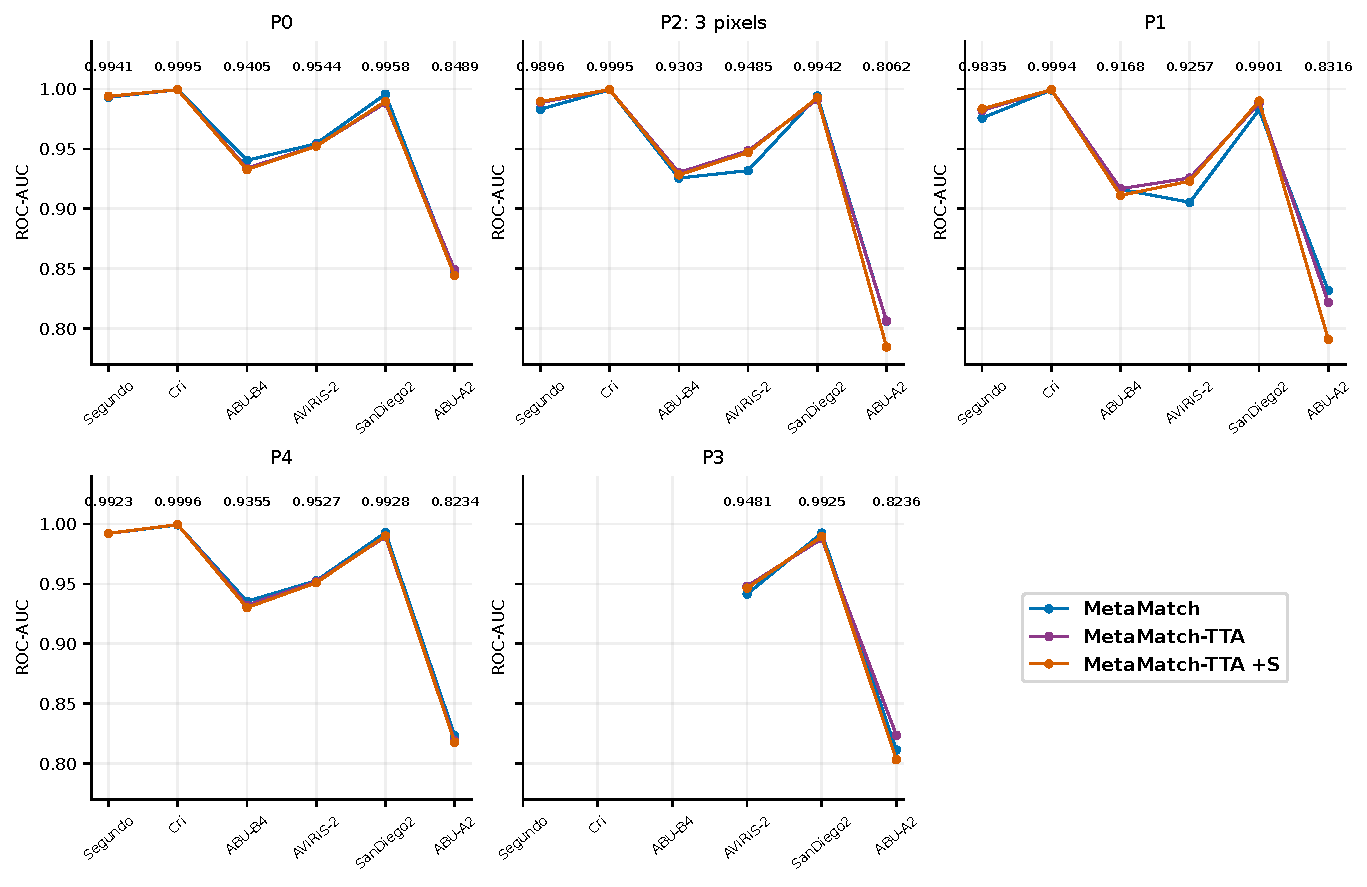
\includegraphics[width=1.0\linewidth]{recent_only_figures/fig_dev.pdf}\caption{Development-scene ROC-AUC under five reference conditions. \textbf{\matcher{}} performs direct matching, \textbf{\method{}} adds reference refinement, and \textbf{\method{} +S} equally averages teacher and student scores. All methods share the reference from the same draw.}\label{full:fig:dev}\end{figure}

Figure~\ref{full:fig:dev} shows output-stage changes on held-out scenes by protocol. On AVIRIS-2, refinement improves P1 and three-pixel-reference results by 2.03 and 1.66 percentage points, respectively, demonstrating supplementation of target information under different observation budgets. Direct matching on SanDiego2 under P4 achieves 0.9928, exceeding the refined result of 0.9895 and showing that tolerance to the prescribed perturbations is already present in the shared network. On ABU-A2 under P2, the two stages achieve 0.8060 and 0.8062, indicating that the effect of additional candidates also depends on initial discrimination quality. The curves distinguish transferable material knowledge from reference supplementation and support combining a fixed matcher with adaptation at the input for new backgrounds.
\FloatBarrier


\section{Complete Results by Reference Protocol and Output Metric}\label{app:protocol_detail}
This section summarizes the complete results of \matcher{}, \method{}, and student fusion by reference construction. P0 provides a benchmark with sufficient target information, P1 and P2 evaluate reference budgets, P4 evaluates the prescribed spectral changes, and P3 evaluates cross-image references. Tables also report run variability, allowing the roles of shared material matching and scene adaptation to be compared within each protocol.






\subsection{Complete Results under Different Reference Protocols}




\begin{table}[H]\centering\footnotesize\setlength{\tabcolsep}{4pt}\renewcommand{\arraystretch}{1.14}
\caption{ROC-AUC of FAME-Net (2026) and our output stages with the P0 ground-truth mean reference. Our entries are means $\pm$ descriptive standard deviations over the unified run set. FAME-Net values are quoted directly from the original paper~\cite{fame}. The highest mean in each row is bold, and +S denotes optional student fusion. The published HYDICE mask and ours contain 19 and 21 target pixels, respectively.}\label{full:tab:p0}
\begin{lrbox}{\fulltablebox}\begin{tabular}{lcccc}\toprule
Scene & \shortstack{FAME-Net (2026)~\cite{fame}\\Published} & \textbf{\matcher{}} & \textbf{\method{}} & \shortstack{\textbf{\method{}}\\+S} \\ \midrule
ABU-A3 & \textbf{0.9916} & \shortstack{0.9791\\$\pm$0.0012} & \shortstack{0.9778\\$\pm$0.0025} & \shortstack{0.9809\\$\pm$0.0015} \\
ABU-B3 & \textbf{1.0000} & \shortstack{0.9910\\$\pm$0.0016} & \shortstack{0.9907\\$\pm$0.0009} & \shortstack{0.9891\\$\pm$0.0027} \\
ABU-U4 & \textbf{0.9980} & \shortstack{0.9975\\$\pm$0.0002} & \shortstack{0.9975\\$\pm$0.0002} & \shortstack{0.9976\\$\pm$0.0002} \\
SanDiego & \textbf{0.9997} & \shortstack{0.9944\\$\pm$0.0015} & \shortstack{0.9954\\$\pm$0.0009} & \shortstack{0.9945\\$\pm$0.0011} \\
HYDICE & \textbf{0.9998} & \shortstack{0.9982\\$\pm$0.0004} & \shortstack{0.9981\\$\pm$0.0006} & \shortstack{0.9976\\$\pm$0.0019} \\
WHR & \textbf{0.9999} & \shortstack{0.9946\\$\pm$0.0010} & \shortstack{0.9946\\$\pm$0.0010} & \shortstack{0.9945\\$\pm$0.0010} \\
\bottomrule\end{tabular}\end{lrbox}\ifdim\wd\fulltablebox>\linewidth\resizebox{\linewidth}{!}{\usebox{\fulltablebox}}\else\usebox{\fulltablebox}\fi\end{table}

Table~\ref{full:tab:p0} reports ranking accuracy with sufficient target information. Macro-average ROC-AUC is 0.9925 for \matcher{} and 0.9924 for \method{}, compared with the published FAME-Net value of 0.9982. Direct matching achieves 0.9975 on ABU-U4 and 0.9982 on HYDICE, showing that material relationships learned during development can be applied directly to new images. Since P0 already aggregates all targets, the average effect of reference refinement is small, consistent with a reduced need for additional observations. This table establishes an accuracy reference with relatively complete target information and, together with limited-reference results, supports the adaptability of the shared matcher to different target descriptions.

\begin{table}[H]\centering\footnotesize\setlength{\tabcolsep}{4pt}\renewcommand{\arraystretch}{1.14}
\caption{ROC-AUC of our output stages with P1 random single-pixel references. All columns use the same three reference draws and three training seeds and report means $\pm$ descriptive standard deviations. The highest mean in each row is bold. +S denotes optional student fusion.}\label{full:tab:p1}
\begin{lrbox}{\fulltablebox}\begin{tabular}{lccc}\toprule
Scene & \textbf{\matcher{}} & \textbf{\method{}} & \shortstack{\textbf{\method{}}\\+S} \\ \midrule
ABU-A3 & \shortstack{0.9747\\$\pm$0.0061} & \shortstack{0.9747\\$\pm$0.0057} & \shortstack{\textbf{0.9781}\\$\pm$0.0050} \\
ABU-B3 & \shortstack{\textbf{0.9865}\\$\pm$0.0094} & \shortstack{0.9850\\$\pm$0.0057} & \shortstack{0.9834\\$\pm$0.0068} \\
ABU-U4 & \shortstack{0.9967\\$\pm$0.0005} & \shortstack{0.9970\\$\pm$0.0004} & \shortstack{\textbf{0.9972}\\$\pm$0.0004} \\
SanDiego & \shortstack{0.9912\\$\pm$0.0032} & \shortstack{0.9914\\$\pm$0.0034} & \shortstack{\textbf{0.9919}\\$\pm$0.0020} \\
HYDICE & \shortstack{0.9916\\$\pm$0.0095} & \shortstack{\textbf{0.9971}\\$\pm$0.0013} & \shortstack{0.9965\\$\pm$0.0027} \\
WHR & \shortstack{\textbf{0.9966}\\$\pm$0.0014} & \shortstack{0.9963\\$\pm$0.0010} & \shortstack{0.9961\\$\pm$0.0011} \\
\bottomrule\end{tabular}\end{lrbox}\ifdim\wd\fulltablebox>\linewidth\resizebox{\linewidth}{!}{\usebox{\fulltablebox}}\else\usebox{\fulltablebox}\fi\end{table}

Table~\ref{full:tab:p1} presents both average accuracy and run variability with single-pixel references. The macro-average of \matcher{} is 0.9895, showing that one measured target spectrum can invoke shared material relationships for ranking. Reference refinement improves HYDICE from $0.9916\pm0.0095$ to $0.9971\pm0.0013$, increasing mean accuracy and stability across runs. ABU-U4 also improves from $0.9967\pm0.0005$ to $0.9970\pm0.0004$. These changes indicate that forming a reference from multiple scene candidates can reduce sensitivity to an individual selection. The two ABU-B3 stages yield 0.9865 and 0.9850, and candidate composition under its extremely sparse target conditions is analyzed in the main paper. Overall, the single-pixel results support material-task learning as the basis for discrimination, supplemented by reference observations through gradient-free updates.

\begin{table}[H]\centering\footnotesize\setlength{\tabcolsep}{4pt}\renewcommand{\arraystretch}{1.14}
\caption{ROC-AUC of our output stages with P2 three-pixel mean references. Reference sampling, seeds, and aggregation follow Table~\ref{full:tab:p1}. The highest mean in each row is bold.}\label{full:tab:p2a}
\begin{lrbox}{\fulltablebox}\begin{tabular}{lccc}\toprule
Scene & \textbf{\matcher{}} & \textbf{\method{}} & \shortstack{\textbf{\method{}}\\+S} \\ \midrule
ABU-A3 & \shortstack{0.9697\\$\pm$0.0153} & \shortstack{0.9665\\$\pm$0.0184} & \shortstack{\textbf{0.9701}\\$\pm$0.0159} \\
ABU-B3 & \shortstack{0.9895\\$\pm$0.0061} & \shortstack{\textbf{0.9899}\\$\pm$0.0038} & \shortstack{0.9886\\$\pm$0.0039} \\
ABU-U4 & \shortstack{0.9967\\$\pm$0.0005} & \shortstack{0.9971\\$\pm$0.0004} & \shortstack{\textbf{0.9973}\\$\pm$0.0003} \\
SanDiego & \shortstack{0.9937\\$\pm$0.0027} & \shortstack{\textbf{0.9946}\\$\pm$0.0021} & \shortstack{0.9939\\$\pm$0.0015} \\
HYDICE & \shortstack{0.9969\\$\pm$0.0016} & \shortstack{\textbf{0.9970}\\$\pm$0.0017} & \shortstack{0.9962\\$\pm$0.0034} \\
WHR & \shortstack{0.9937\\$\pm$0.0022} & \shortstack{\textbf{0.9942}\\$\pm$0.0012} & \shortstack{\textbf{0.9942}\\$\pm$0.0010} \\
\bottomrule\end{tabular}\end{lrbox}\ifdim\wd\fulltablebox>\linewidth\resizebox{\linewidth}{!}{\usebox{\fulltablebox}}\else\usebox{\fulltablebox}\fi\end{table}

Table~\ref{full:tab:p2a} tests whether scene candidates remain useful after averaging a few observations. With three-pixel references, \method{} exceeds direct \matcher{} in five of six scenes. SanDiego improves from 0.9937 to 0.9946, and WHR from 0.9937 to 0.9942. Even when the initial reference contains multiple observations, updates can add useful image information, so their role extends beyond replacing a single pixel. On ABU-A3, the result changes from 0.9697 to 0.9665, leaving the macro-average of 0.9899 slightly below the direct value of 0.9900. Both reference coverage and candidate quality determine the benefit. The results support combining few-pixel mean references and scene observations through the same pairwise interface for adaptation under different target-information budgets.

\begin{table}[H]\centering\footnotesize\setlength{\tabcolsep}{4pt}\renewcommand{\arraystretch}{1.14}
\caption{ROC-AUC of our output stages with P2 five-pixel mean references. Reference sampling, seeds, and aggregation follow Table~\ref{full:tab:p1}. The highest mean in each row is bold.}\label{full:tab:p2b}
\begin{lrbox}{\fulltablebox}\begin{tabular}{lccc}\toprule
Scene & \textbf{\matcher{}} & \textbf{\method{}} & \shortstack{\textbf{\method{}}\\+S} \\ \midrule
ABU-A3 & \shortstack{\textbf{0.9812}\\$\pm$0.0010} & \shortstack{0.9797\\$\pm$0.0029} & \shortstack{0.9808\\$\pm$0.0026} \\
ABU-B3 & \shortstack{0.9899\\$\pm$0.0028} & \shortstack{\textbf{0.9901}\\$\pm$0.0015} & \shortstack{0.9879\\$\pm$0.0038} \\
ABU-U4 & \shortstack{0.9966\\$\pm$0.0004} & \shortstack{0.9971\\$\pm$0.0004} & \shortstack{\textbf{0.9973}\\$\pm$0.0003} \\
SanDiego & \shortstack{0.9943\\$\pm$0.0019} & \shortstack{\textbf{0.9954}\\$\pm$0.0013} & \shortstack{0.9944\\$\pm$0.0013} \\
HYDICE & \shortstack{0.9962\\$\pm$0.0031} & \shortstack{\textbf{0.9974}\\$\pm$0.0016} & \shortstack{0.9966\\$\pm$0.0028} \\
WHR & \shortstack{\textbf{0.9948}\\$\pm$0.0013} & \shortstack{\textbf{0.9948}\\$\pm$0.0012} & \shortstack{0.9944\\$\pm$0.0014} \\
\bottomrule\end{tabular}\end{lrbox}\ifdim\wd\fulltablebox>\linewidth\resizebox{\linewidth}{!}{\usebox{\fulltablebox}}\else\usebox{\fulltablebox}\fi\end{table}

In Table~\ref{full:tab:p2b}, \method{} achieves a five-pixel macro-average ROC-AUC of 0.9924, matching the complete-target-mean result at the reported precision. SanDiego achieves 0.9954 with both five-pixel and P0 references, while ABU-U4 achieves 0.9971 and 0.9975, respectively. On ABU-A3, accuracy increases from the three-pixel value of 0.9665 to 0.9797, and the standard deviation decreases from 0.0184 to 0.0029. More observations improve the mean while reducing variability from sampling and training. Network weights remain unchanged, and additional information enters only through the reference vector. These results support compatibility with different observation counts through randomized-reference task training, allowing a few target samples to approach full-reference detection performance.

\begin{table}[H]\centering\footnotesize\setlength{\tabcolsep}{4pt}\renewcommand{\arraystretch}{1.14}
\caption{ROC-AUC of our output stages with P4 synthetically perturbed references. Reference sampling, seeds, and aggregation follow Table~\ref{full:tab:p1}. The highest mean in each row is bold.}\label{full:tab:p4}
\begin{lrbox}{\fulltablebox}\begin{tabular}{lccc}\toprule
Scene & \textbf{\matcher{}} & \textbf{\method{}} & \shortstack{\textbf{\method{}}\\+S} \\ \midrule
ABU-A3 & \shortstack{0.9725\\$\pm$0.0080} & \shortstack{0.9738\\$\pm$0.0073} & \shortstack{\textbf{0.9751}\\$\pm$0.0074} \\
ABU-B3 & \shortstack{\textbf{0.9901}\\$\pm$0.0035} & \shortstack{0.9839\\$\pm$0.0064} & \shortstack{0.9797\\$\pm$0.0102} \\
ABU-U4 & \shortstack{0.9974\\$\pm$0.0003} & \shortstack{0.9974\\$\pm$0.0003} & \shortstack{\textbf{0.9976}\\$\pm$0.0003} \\
SanDiego & \shortstack{\textbf{0.9955}\\$\pm$0.0014} & \shortstack{0.9940\\$\pm$0.0014} & \shortstack{0.9932\\$\pm$0.0016} \\
HYDICE & \shortstack{\textbf{0.9977}\\$\pm$0.0016} & \shortstack{\textbf{0.9977}\\$\pm$0.0010} & \shortstack{0.9974\\$\pm$0.0020} \\
WHR & \shortstack{\textbf{0.9951}\\$\pm$0.0012} & \shortstack{0.9950\\$\pm$0.0010} & \shortstack{0.9948\\$\pm$0.0011} \\
\bottomrule\end{tabular}\end{lrbox}\ifdim\wd\fulltablebox>\linewidth\resizebox{\linewidth}{!}{\usebox{\fulltablebox}}\else\usebox{\fulltablebox}\fi\end{table}

Table~\ref{full:tab:p4} tests matching under the combined prescribed gain changes, smooth deformations, and noise. Direct \matcher{} achieves a macro-average ROC-AUC of 0.9914, only 0.11 percentage points below its P0 value of 0.9925. Its results on ABU-U4 and HYDICE are 0.9974 and 0.9977, close to their P0 values of 0.9975 and 0.9982. The shared network therefore retains a basis for ranking target materials when reference values change. \method{} has a macro-average of 0.9903, with ABU-B3 changing from the direct result of 0.9901 to 0.9839, emphasizing the strong discrimination already present in initial matching under this protocol. Together with the augmentation ablation, these results support explicitly covering spectral changes during training so that tolerance to the prescribed perturbation families becomes part of the shared matching function.

\begin{table}[H]\centering\footnotesize\setlength{\tabcolsep}{4pt}\renewcommand{\arraystretch}{1.14}
\caption{ROC-AUC of our output stages with P3 cross-image references. Donor--target pairs are ABU-A2 $\to$ ABU-A3, ABU-A3 $\to$ ABU-U4, and SanDiego2 $\to$ SanDiego. Results average three training seeds, with the highest mean in each row in bold.}\label{full:tab:p3}
\begin{lrbox}{\fulltablebox}\begin{tabular}{lccc}\toprule
Scene & \textbf{\matcher{}} & \textbf{\method{}} & \shortstack{\textbf{\method{}}\\+S} \\ \midrule
ABU-A3 & \shortstack{\textbf{0.9783}\\$\pm$0.0011} & \shortstack{0.9746\\$\pm$0.0048} & \shortstack{0.9781\\$\pm$0.0027} \\
ABU-U4 & \shortstack{0.9940\\$\pm$0.0016} & \shortstack{0.9949\\$\pm$0.0013} & \shortstack{\textbf{0.9955}\\$\pm$0.0011} \\
SanDiego & \shortstack{\textbf{0.9949}\\$\pm$0.0014} & \shortstack{0.9928\\$\pm$0.0008} & \shortstack{0.9926\\$\pm$0.0011} \\
\bottomrule\end{tabular}\end{lrbox}\ifdim\wd\fulltablebox>\linewidth\resizebox{\linewidth}{!}{\usebox{\fulltablebox}}\else\usebox{\fulltablebox}\fi\end{table}

Table~\ref{full:tab:p3} evaluates exploratory matching with references from another image when band layouts are compatible. Direct \matcher{} achieves a macro-average of 0.9891 over the three pairs, and \method{} achieves 0.9874. ABU-U4 uses a reference from ABU-A3 and improves from 0.9940 to 0.9949 after refinement, showing that current-image candidates can beneficially adjust an external reference. This input requires no network retraining, demonstrating reuse of the reference--query pairing interface. Refined results on ABU-A3 and SanDiego are lower than direct matching. The scope of material-identity verification for these pairs is specified in the protocol definition. This experiment provides preliminary evidence for combining a fixed network with target-image background statistics and an external reference, supporting adaptation focused on references and statistical conditions.

\begin{figure}[H]\centering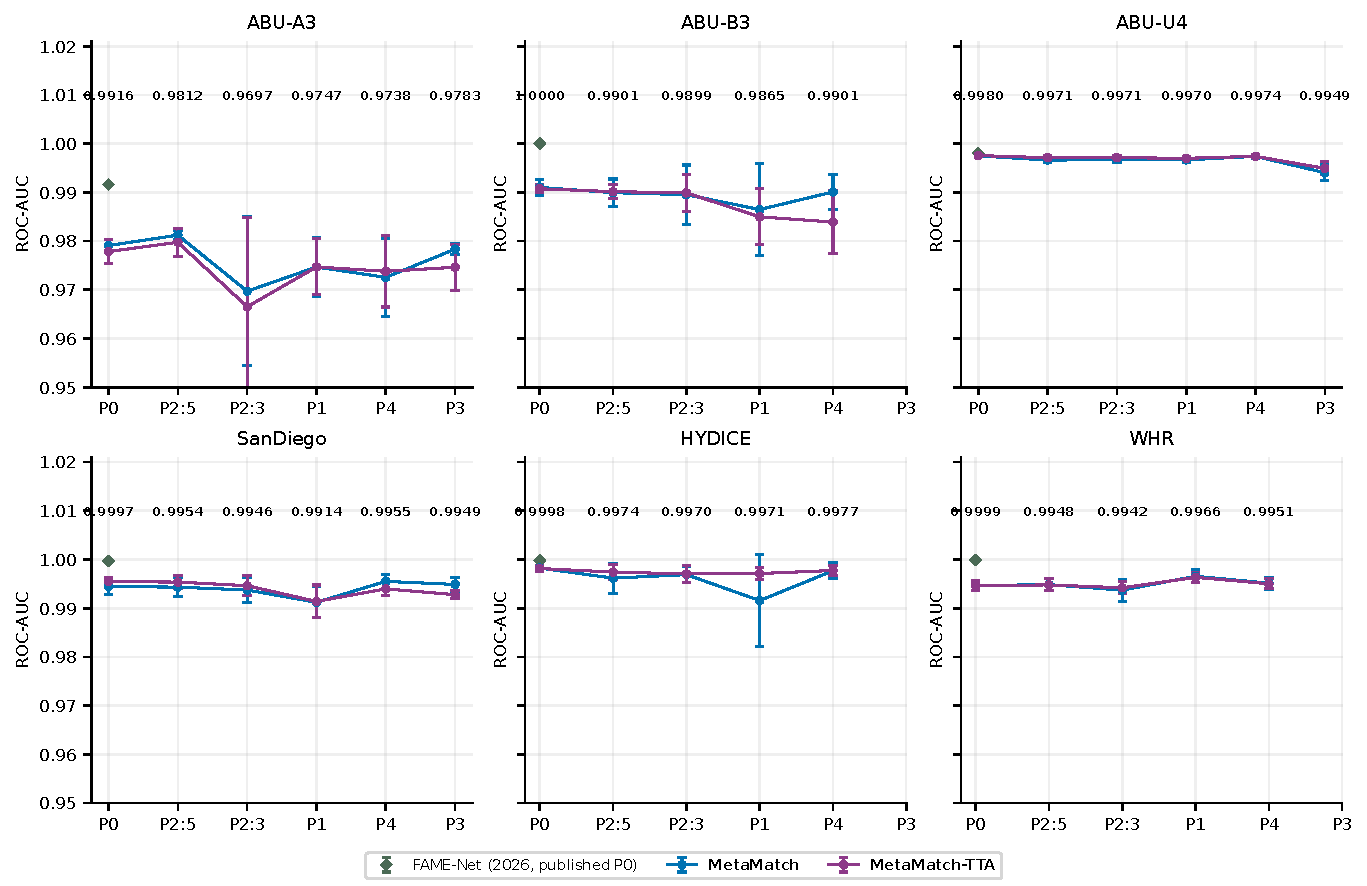
\includegraphics[width=1.0\linewidth]{recent_only_figures/fig_targets_auc1.pdf}\caption{Scene-specific ROC-AUC of \matcher{}, \method{}, and FAME-Net (2026) under six reference settings. FAME-Net is plotted only under P0 using published values~\cite{fame}. Our error bars show descriptive standard deviations. The highest plotted mean for each scene and protocol is bold. The published HYDICE mask and ours contain 19 and 21 target pixels, respectively.}\label{full:fig:targets}\end{figure}

Figure~\ref{full:fig:targets} jointly presents reference conditions and scene differences to examine the image-level basis of macro-average performance. Under single-pixel, three-pixel, five-pixel, and complete-mean references, \method{} achieves 0.9970--0.9975 on ABU-U4 and 0.9970--0.9981 on HYDICE. Both target types retain high ranking accuracy as reference information changes. ABU-A3 achieves 0.9665 and 0.9797 with three- and five-pixel references, illustrating the benefit of more complete target observations in this scene. P0 also includes published FAME-Net values, while the other protocols show our means and variability. The scene-specific results show that the same pairing rules can preserve high accuracy in some scenes and exploit added reference information in others, providing detailed support for shared-network processing of different target descriptions.

\begin{figure}[H]\centering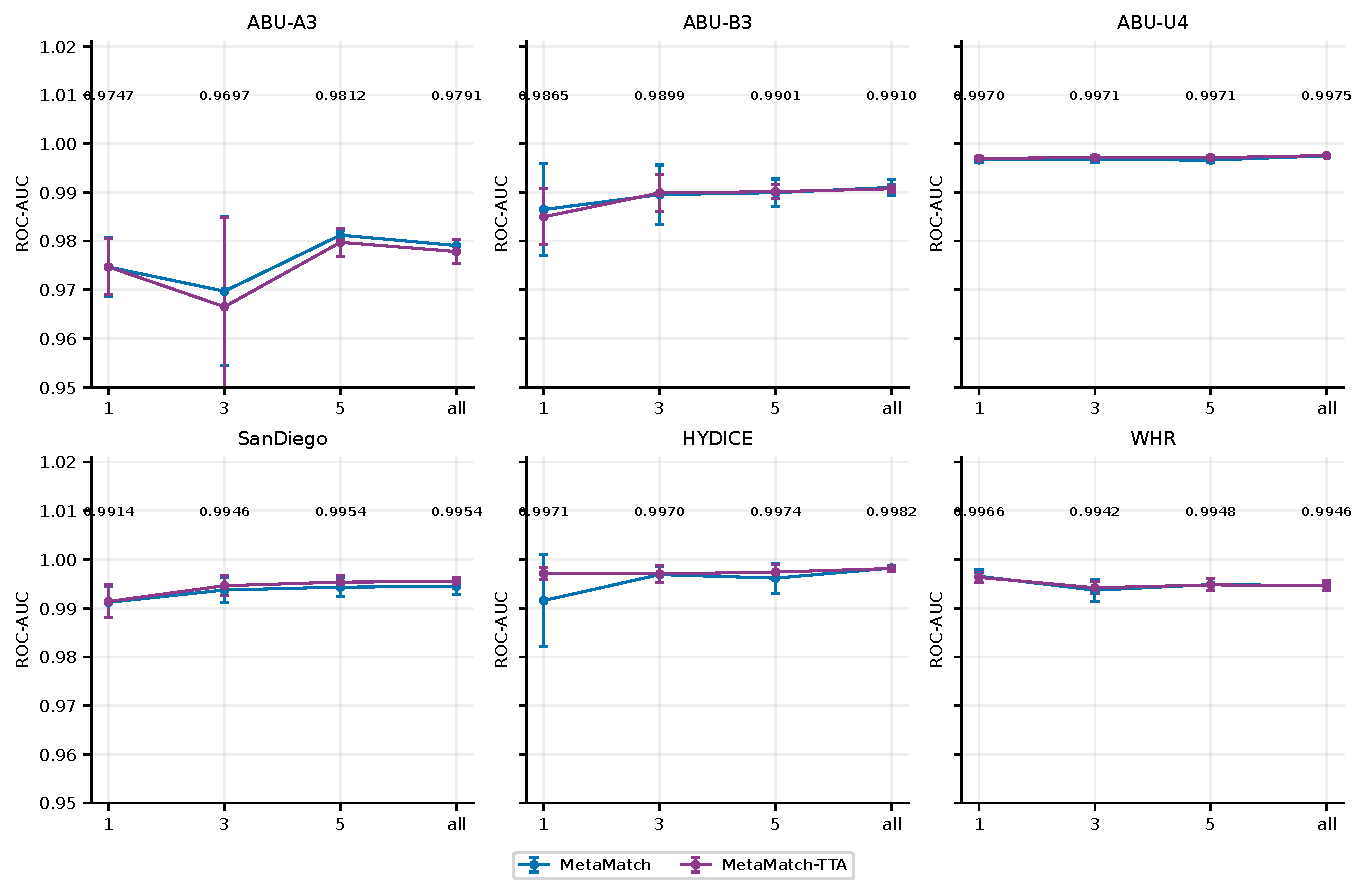
\includegraphics[width=1.0\linewidth]{recent_only_figures/fig_sens_k.pdf}\caption{Effect of reference target-pixel count on the ROC-AUC of \matcher{} and \method{}. References use one, three, five, or all target pixels. Error bars show descriptive standard deviations, and the higher mean at each setting is bold. ``all'' denotes the mean of the complete target region.}\label{full:fig:sensk}\end{figure}

Figure~\ref{full:fig:sensk} examines whether changes in reference budget require model redesign or retraining. The macro-average ROC-AUC of \method{} ranges from 0.9899 to 0.9924 as the reference grows from one pixel to all target pixels. Both five-pixel and complete-mean references achieve 0.9924, showing that limited observations already approach full-reference overall ranking. ABU-A3 varies more with three pixels, while five pixels increase accuracy and narrow error bars. A larger budget thus improves reference coverage and representativeness. ABU-U4 remains similar across these budgets, indicating that the shared matcher can extract useful relationships from fewer observations. The figure supports adaptation to input-information quantity through randomized-reference training. Reference count changes at the input while the prediction head and network weights are reused.

Figure~\ref{fig:protocols} summarizes the effects of reference count, spectral perturbation, and reference source on the shared matcher. \method{} achieves 0.9902 under P1 and 0.9903 under P4, close to its P0 value of 0.9924. Neither an insufficient individual observation nor the prescribed spectral variation causes a large overall loss of ranking ability. Five-pixel references restore 0.9924, while direct matching achieves 0.9914 under P4, showing the separate roles of added target information and previously learned tolerance to variation. P3 summarizes three exploratory pairs, and FAME-Net supplies a published reference only for P0. The figure supports a unified matching formulation across reference conditions, with shared relationships and adaptation through input conditions jointly maintaining detection capability.

\begin{figure}[htbp]\centering
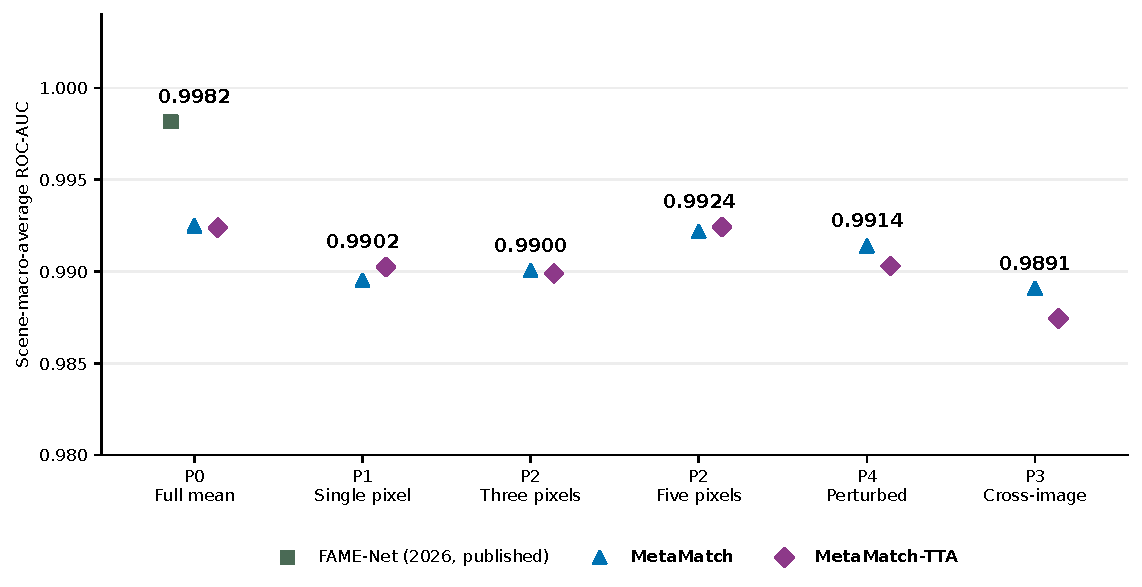
\includegraphics[width=.85\linewidth]{english_figures/protocol_comparison.pdf}
\caption{Macro-average ROC-AUC of \matcher{} and \method{} under different reference protocols. FAME-Net (2026) is plotted only for P0 using published values~\cite{fame}. The highest plotted mean within each protocol is bold. P3 contains three image pairs, and the other protocols contain six scenes.}\label{fig:protocols}
\end{figure}

P4 starts from the complete target mean and uses variation families overlapping with training augmentation, primarily evaluating tolerance to the prescribed spectral changes. P1 samples real target pixels randomly and primarily evaluates the representativeness of an individual observation. These protocols examine reference insufficiency from different directions. Together with augmentation ablations, they support varying both reference observations and spectral forms within training tasks.

\subsection{Five Metrics for the Output Stages}
\begin{table}[H]\centering\footnotesize\setlength{\tabcolsep}{4pt}\renewcommand{\arraystretch}{1.14}
\caption{Five AUC metrics of \method{} and \method{} +S after an $s^4$ transformation under P1. The better value for each metric within each scene is bold. Lower AUC$_2$ and higher values of the other metrics are preferred. The outputs differ in both model stage and score transformation.}\label{full:tab:p1five}
\begin{lrbox}{\fulltablebox}\begin{tabular}{lcccccc}\toprule
Scene & Method & AUC$_1\uparrow$ & AUC$_2\downarrow$ & AUC$_3\uparrow$ & AUC$_4\uparrow$ & AUC$_5\uparrow$ \\ \midrule
ABU-A3 & \textbf{\method{}} & 0.9747 & 0.0879 & \textbf{0.7169} & \textbf{1.6037} & 8.4 \\
 & \shortstack{\textbf{\method{}}\\+S, $s^4$} & \textbf{0.9781} & \textbf{0.0113} & 0.3553 & 1.3221 & \textbf{32.7} \\
ABU-B3 & \textbf{\method{}} & \textbf{0.9850} & 0.0806 & \textbf{0.8010} & \textbf{1.7054} & 10.3 \\
 & \shortstack{\textbf{\method{}}\\+S, $s^4$} & 0.9834 & \textbf{0.0115} & 0.5494 & 1.5213 & \textbf{51.6} \\
ABU-U4 & \textbf{\method{}} & 0.9970 & 0.0174 & \textbf{0.8689} & \textbf{1.8485} & 50.9 \\
 & \shortstack{\textbf{\method{}}\\+S, $s^4$} & \textbf{0.9972} & \textbf{0.0048} & 0.6226 & 1.6149 & \textbf{131.5} \\
SanDiego & \textbf{\method{}} & 0.9914 & 0.0893 & \textbf{0.9158} & \textbf{1.8178} & 10.4 \\
 & \shortstack{\textbf{\method{}}\\+S, $s^4$} & \textbf{0.9919} & \textbf{0.0269} & 0.7021 & 1.6671 & \textbf{26.2} \\
HYDICE & \textbf{\method{}} & \textbf{0.9971} & 0.0811 & \textbf{0.9067} & \textbf{1.8227} & 11.8 \\
 & \shortstack{\textbf{\method{}}\\+S, $s^4$} & 0.9965 & \textbf{0.0034} & 0.7040 & 1.6972 & \textbf{227.1} \\
WHR & \textbf{\method{}} & \textbf{0.9963} & 0.1981 & \textbf{0.9463} & 1.7445 & 5.5 \\
 & \shortstack{\textbf{\method{}}\\+S, $s^4$} & 0.9961 & \textbf{0.0303} & 0.8161 & \textbf{1.7820} & \textbf{28.6} \\
\bottomrule\end{tabular}\end{lrbox}\ifdim\wd\fulltablebox>\linewidth\resizebox{\linewidth}{!}{\usebox{\fulltablebox}}\else\usebox{\fulltablebox}\fi\end{table}

Table~\ref{full:tab:p1five} evaluates ranking and score responses jointly. On ABU-U4, moving from \method{} to student fusion followed by $s^4$ changes AUC$_1$ from 0.9970 to 0.9972, decreases AUC$_2$ from 0.0174 to 0.0048, and decreases AUC$_3$ from 0.8689 to 0.6226. Background and target responses are compressed together, concentrating the output distribution in the low-score region. The configurations differ in both model stage and score transformation. High ranking accuracy already exists in the original matching output, supporting material-relationship learning as the central design.






\FloatBarrier


\FloatBarrier
\begingroup\footnotesize
\begin{thebibliography}{99}
\bibitem[5]{fame} Z. Yang, M. Zhang, J. Wang, Y. Gao, W. Liao, and W. Li, ``A Dual-Network Framework With Adversarial GMM Augmentation and Frequency-Mamba Fusion for Hyperspectral Target Detection,'' \emph{IEEE Transactions on Neural Networks and Learning Systems}, vol. 37, no. 10, pp. 5090--5104, 2026. \href{https://doi.org/10.1109/TNNLS.2026.3682921}{doi: 10.1109/TNNLS.2026.3682921}.
\end{thebibliography}
\endgroup

\end{document}
